\section{Nixtla Neural Forecast TimeLLM}
{{\footnotesize
\begin{description}[labelwidth=5em, labelsep=1em, leftmargin=*, align=left, itemsep=0.3em, parsep=0em]
  \item[date:] 2023-10-03
  \item[version:] TODO
  \item[last\_updated:] 2025-06
  \item[expired:] unknown
  \item[valid:] yes
  \item[valid\_date:] TODO
  \item[url:] \href{https://github.com/Nixtla/neuralforecast}{https://github.com/Nixtla/neuralforecast}
  \item[doi:] TODO
  \item[domain:] Time-series; General ML
  \item[focus:] Reprogramming LLMs for time series forecasting
  \item[keywords:]
    - Time-LLM
    - language model
    - time-series
    - reprogramming
  \item[summary:] Time-LLM uses reprogramming layers to adapt frozen LLMs for time series forecasting, treating
forecasting as a language task :contentReference[oaicite:2]\{index=2\}.

  \item[licensing:] TODO
  \item[task\_types:]
    - Time-series forecasting
  \item[ai\_capability\_measured:]
    - Model reuse via LLM
    - few-shot forecasting
  \item[metrics:]
    - RMSE
    - MAPE
  \item[models:]
    - Time-LLM
  \item[ml\_motif:]
    - Time-series
  \item[type:] Platform
  \item[ml\_task:]
    - Forecasting
  \item[solutions:] TODO
  \item[notes:] Fully open-source; transforms forecasting using LLM text reconstruction.

  \item[contact.name:] Ming Jin (Nixtla)
  \item[contact.email:] unknown
  \item[datasets.links.name:] Standard forecast datasets, M4
  \item[results.links.name:] ChatGPT LLM
  \item[fair.reproducible:] Yes
  \item[fair.benchmark\_ready:] Yes
  \item[ratings.software.rating:] 0
  \item[ratings.software.reason:] Not analyzed.

  \item[ratings.specification.rating:] 7.0
  \item[ratings.specification.reason:] Describes forecasting with LLMs, but less formal on input/output or task framing.

  \item[ratings.dataset.rating:] 6.0
  \item[ratings.dataset.reason:] Uses open time series datasets, but lacks a consolidated data release or splits.

  \item[ratings.metrics.rating:] 7.0
  \item[ratings.metrics.reason:] Reports metrics like MASE and SMAPE, standard in forecasting.

  \item[ratings.reference\_solution.rating:] 6.0
  \item[ratings.reference\_solution.reason:] Provides TimeLLM with open source, but no other baselines included.

  \item[ratings.documentation.rating:] 6.0
  \item[ratings.documentation.reason:] GitHub readme with installation and example usage; lacks API or extensive tutorials.

  \item[id:] nixtla\_neural\_forecast\_timellm
  \item[Citations:] \cite{jin2024timellmtimeseriesforecasting}
  \item[Ratings:]
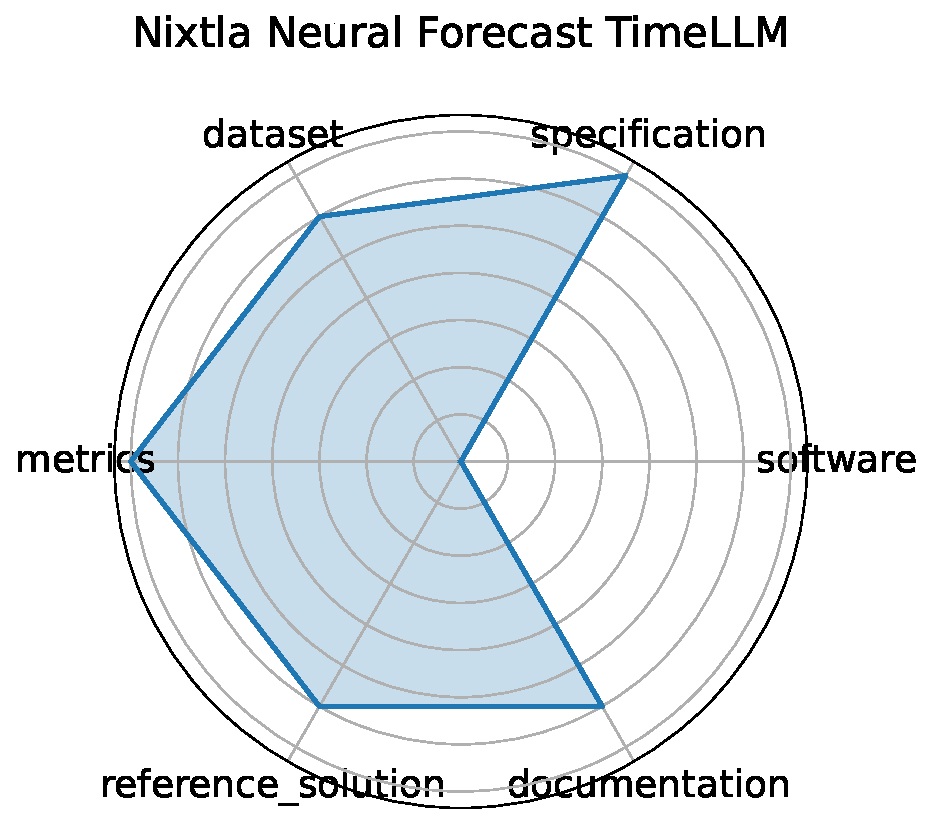
\includegraphics[width=0.2\textwidth]{nixtla_neural_forecast_timellm_radar.pdf}
\end{description}
}}
\clearpage